\chapter{Wstęp teoretyczny}



\section{Historia i stan obecny dziedziny}
Dynamiczny rozwój grafiki komputerowej obserwujemy od roku 1950 kiedy to w Massachusets Institute of Technology [3] powstał pierwszy
komputer wyposażony w grafoskop. Obecnie większość użytkowników nie potrafi sobie wyobrazić komputera bez graficznego interfejsu.
Coraz większe możliwości nowoczesnych komputerów są motorem napędowym rozmaitych badań nad komputerowymi modelami świata rzeczywistego.
Prekursorem w dziedzinie wizualizacji drzew był polski matematyk Stanisław Ulam, przedstawiajac w 1962r[5] drzewo jako samoorganizującą się
strukturę. Jego model wykorzystujący automaty komórkowe opierał się na rywalizacji węzłów  drzewa o przestreń.
Honda zaproponował w 1971r. modelowanie drzew jako stuktury rekursywnej opisanej
zbiorem parametrów takich jak kąt rozgałęzień, czy stosunek długości między kolejnymi poziomami rekurencji[4]. Dopiero w latach osiemdziesiatych
możliwości uwczesnych komputerów pozwoliły na trójwymiarową wizualizację drzew, czego przykładem może być praca Bloomenthala z 85r \cite{bloomenthal}
przedstawiająca proces modelowania klonu. Podejście do tematu możemy podzielić na dwie grupy:
\begin{itemize}
\item od ogółu do szczegółu, czyli modelowanie z zadanymi parametrami wyglądu drzewa
\item od szczegółu do ogółu, czyli opisanie pewnym zbiorem parametrów budowy drzewa
\end{itemize}
Problem stworzenia modelu drzewa możemy podzielić na stworzenie modelów jego składowych np gałęzi, kory, liści, czy kwiatów i późniejsze
ich połączenie w jedną całość. Na chwilę obecną istnieją zaawansowane metody generowania zarówno całych drzew, jak i poszczególnych jego części.

\section{Algorytm kolonizacyjny}
Algorytm kolonizacji przestrzeni dalej nazywany algorytmem kolonizacyjnym opiera się na biologicznym aspekcie rywalizacji roślin o dostępną wokół nich przestrzeń. Po raz pierwszy został zaprezentowany w 2007 roku [1], będąc rozszerzeniem na przestrzeń trójwymiarową metody generowania liści przy wykorzystaniu systemów cząsteczkowych [2]. Podstawową ich ideą było umieszczanie cząstek w obrysie liścia, a następnie śledzenie ich ruchu w kierunku szypułki uwzględniając wzajemne przyciąganie cząstek. Z biologicznego punktu widzenia miało to uzasadnienie jako śledzenie trasy transportu substancji niezbędnych do życia rośliny. W podejściu kolonizacyjnym symuluje się iteracyjny wzrost gałęzi drzewa, aż do wykorzystania całego dostępnego miejsca.


Słowniczek:\\
węzeł drzewa - odcinek w przestrzeni trójwymiarowej reprezentujący część gałęzi\\
atraktor - pkt w przestrzeni trójwymiarowej, do którego osiągniecia dążą węzły drzewa\\
korona - podzbiór punktów przestrzeni trójwymiarowej\\

Dane algorytmu: \\
korona, zbior parametrow: \\
dist(a,b) - funkcja zwracająca odległość euklidesową między dwoma punktami przestrzeni  \\
\begin{verbatim}
  rozmieść atraktory wewnątrz korony drzewa
  dodaj do drzewa wezel glowny
  dopóki istnieją atraktory:
    dla kazdego atraktora a :
      wyznacz najbliższy węzeł drzewa n
       jesli dist(n,a) <=di
        oblicz wektor n->a
      dodaj nowy wezel do drzewa (n-a)
  dla kazdego atraktora
    jesli istnieje wezel drzewa w odleglosci <=dk
      usun atraktor
\end{verbatim}
Parametry: \\
di - influence distance\\
dk - kill distance\\
D - node length\\
points - liczba atraktorów\\

Ponieważ istnieją parametry uniemożliwiające zakonczenie algorytmu np dk<<D warunek konca obliczen na potrzeby implementacji został zastąpiony sprawdzeniem, czy w poprzedniej iteracji został utworzony jakiś nowy węzeł drzewa.
\section{Tworzenie geometrii modelu}
\subsection{Wstęp}
Rośliny, w szczególności drzewa, są bardzo złożonymi strukturami. Projektując model drzewa trzeba zwrócić uwagę na wiele aspektów takich jak: sposób łączenia gałęzi, rozłożenie liści na drzewie, położenie pojedynczego liścia w przestrzeni, sposób przyłączenie liścia do gałęzi.


\subsection{Model węzła}
Węzeł jest opisywny przez położenie(P) oraz promień(R). Na ich podstawie wyliczany jest segment. Segment jest zbiorem przynajmniej 3 punktów leżących na okręgu o środku w punkcie P i promieniu R. Normalna do płaszczyzny tworzonej przez punkty segmentu oraz punkt P jest wyliczana w następujący sposób: $\vec{n}=\frac{\vec{AP}}{\abs{AP}}+\frac{\vec{PB}}{\abs{PB}}$, gdzie A - poprzednik P; B - następnik P. Jeśli węzeł A lub B nie istnieje, to odpowiednio pierwszy lub drugi składnik sumy przyjmuje wartość 0.

TODO wyznaczanie promienia węzła.

\begin{center}
	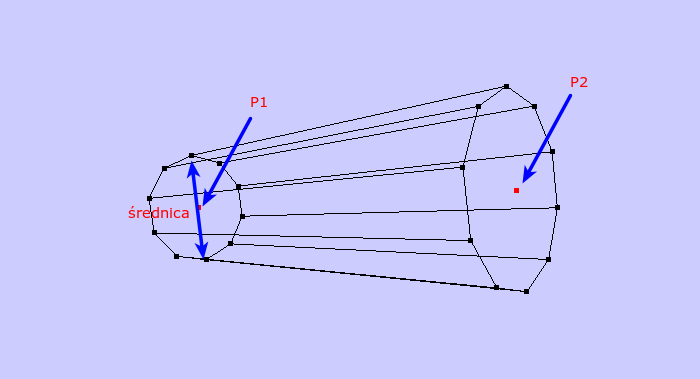
\includegraphics[width=100mm]{images/model/two_segments.png}
	\captionof{figure}{Dwa wyrenderowane segmenty wokół węzłów P1 i P2}
	\label{two_segments}
\end{center}

\subsection{Model gałęzi}
Dobrym przybliżeniem gałęzi jest uogólniony walec (ang. generalized cylinder). Jest to powierzchnia w przestrzeni $R^3$, której przekrój poprzeczny jest krzywą zamkniętą.

Gałąź jest reprezentowana przez listę kolejnych węzłów. Węzeł o najniższym indeksie znajduje się na początku gałęzi(rozwidlenie bądź początek drzewa). Aby gałąź utworzyła uogólniony walec, łączymy ze sobą odpowiednie punkty segmentów sąsiednich węzłów (rys. \ref{two_segments} oraz \ref{branching}).

Gałąź może być początkiem kolejnych konarów, dlatego posiada kolekcję gałęzi potomnych.

TODO wyznaczanie gałęzi.

\begin{center}
	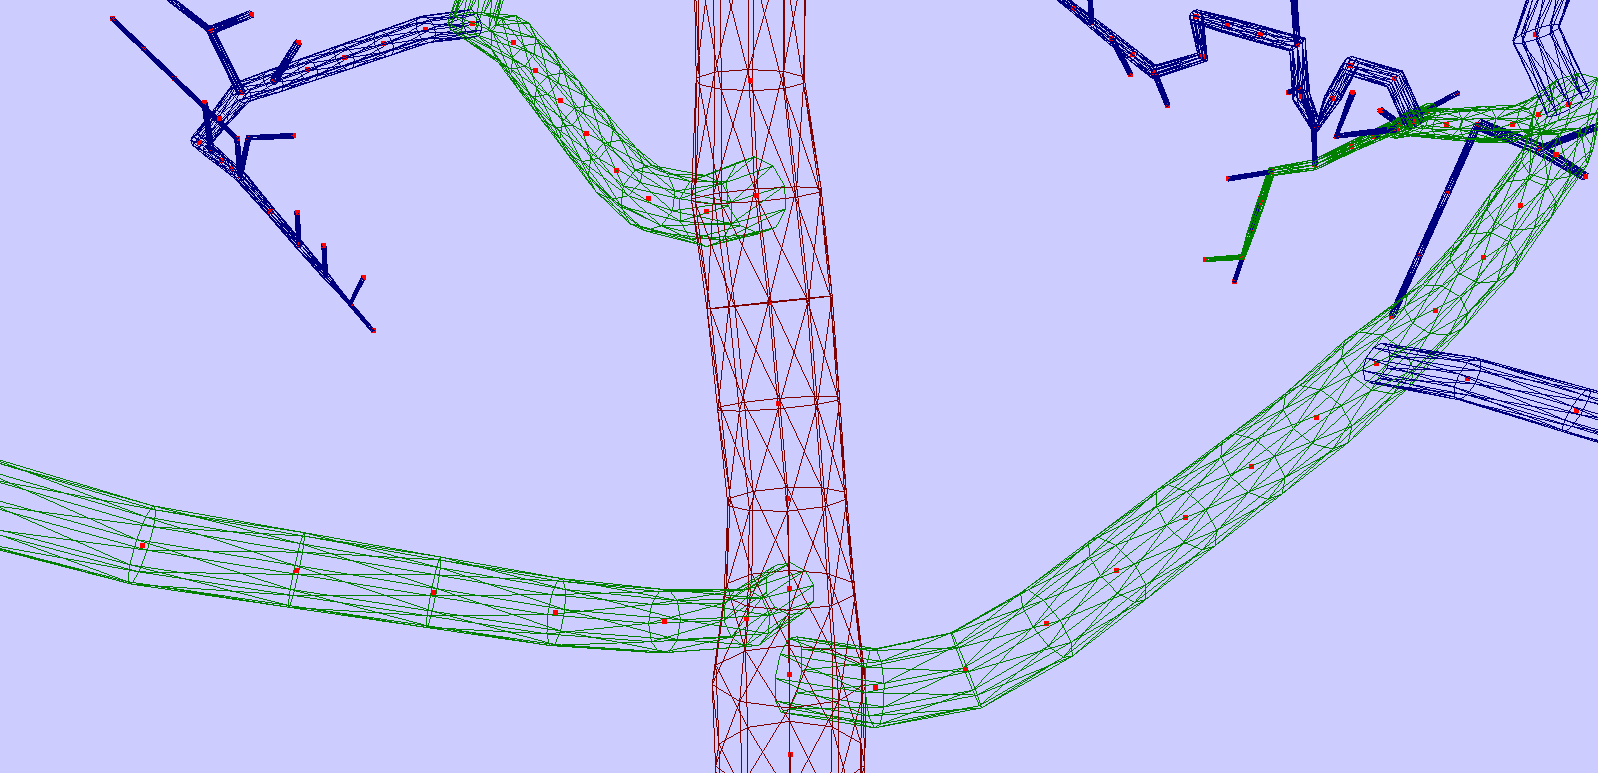
\includegraphics[width=130mm]{images/model/branching.png}
	\captionof{figure}{Łączenie gałęzi.}
	\label{branching}
\end{center}
\subsection{Model liścia}
Liść cechuje się dwiema właściwościami: normalną do powierzchnii liścia oraz wektorem wyznaczającym kierunek liścia. Oba wektory są do siebie prostopadłe.

TODO rysunek z liściem i wektorami.

\section{Teksturowanie}
